\documentclass{beamer}
\usepackage{fontspec}
\usepackage[russian]{babel}
\usepackage{csquotes}
\usepackage{gost-table}
\usepackage{graphicx}
\usepackage{amsmath}
\usepackage{multicol}
\usepackage{float}
\usepackage{wrapfig}

%%% beamer
\setmainfont{Times New Roman}
\usefonttheme{serif}
\usetheme{boxes}
\beamertemplatenavigationsymbolsempty
\setbeamertemplate{frametitle}[default][center]
\setbeamertemplate{footline}[page number]
%%%

\begin{document}
\begin{frame}
    \begin{center}
        Липецкий государственный технический университет\\
        Кафедра автоматизированных систем управления
        \vfill
        \uppercase{ВЫПУСКНАЯ КВАЛИФИКАЦИОННАЯ РАБОТА БАКАЛАВРА}\\
        по направлению 09.03.04 \textquote{Программная инженерия}\\
        \textquote{%
            Разработка информационной системы поддержки технического
            обслуживания автомобильного парка%
        }
    \end{center}
    \vfill
    \begin{tabularx}{\textwidth}{Lm{4cm}R}
        Студент & & Федин М.С. \\
        Группа ПИ-18 & & \\
        Руководитель & & \\
        к.т.н., доцент & & Назаркин О.А.
    \end{tabularx}
\end{frame}

\begin{frame}
    {Характеристика предметной области}
    В процессе эксплуатации автомобиля его составные части изнашиваются, что
    приводит к снижению эффективности или даже поломке.
    \\[\baselineskip]

    Существует два способа поддержания работоспособности автомобиля:
    \begin{itemize}
        \item техническое обслуживание (ТО);
        \item ремонт (Р).
    \end{itemize}
\end{frame}

\begin{frame}
	{Постановка задачи и критерии успешности системы}
    Упрощение задачи поддержки автомобильного парка в технически исправном
    состоянии можно достичь путем ведения единой информационной базы по всем
    машинам.
    \\[\baselineskip]

    Основными факторами успешности разрабатываемой системы являются качество
    технического состояния автомобильной техники, а также снижение затрат при
    проведении работ.
\end{frame}

\begin{frame}
	{Функции системы}
    \begin{itemize}
      \item учет текущего статуса проведения технического обслуживания автомобилей;
      \item учет активных задач автослесаря;
      \item учет ресурсов, необходимых для проведения ТО;
      \item генерация отчетов о затратах за период времени, указываемый
          пользователем;
      \item помощь в составлении графика прохождения технического обслуживания
          техники.
    \end{itemize}
\end{frame}

\begin{frame}
	{ER-диаграмма предметной области}
    \begin{figure}[h]
        \centering
        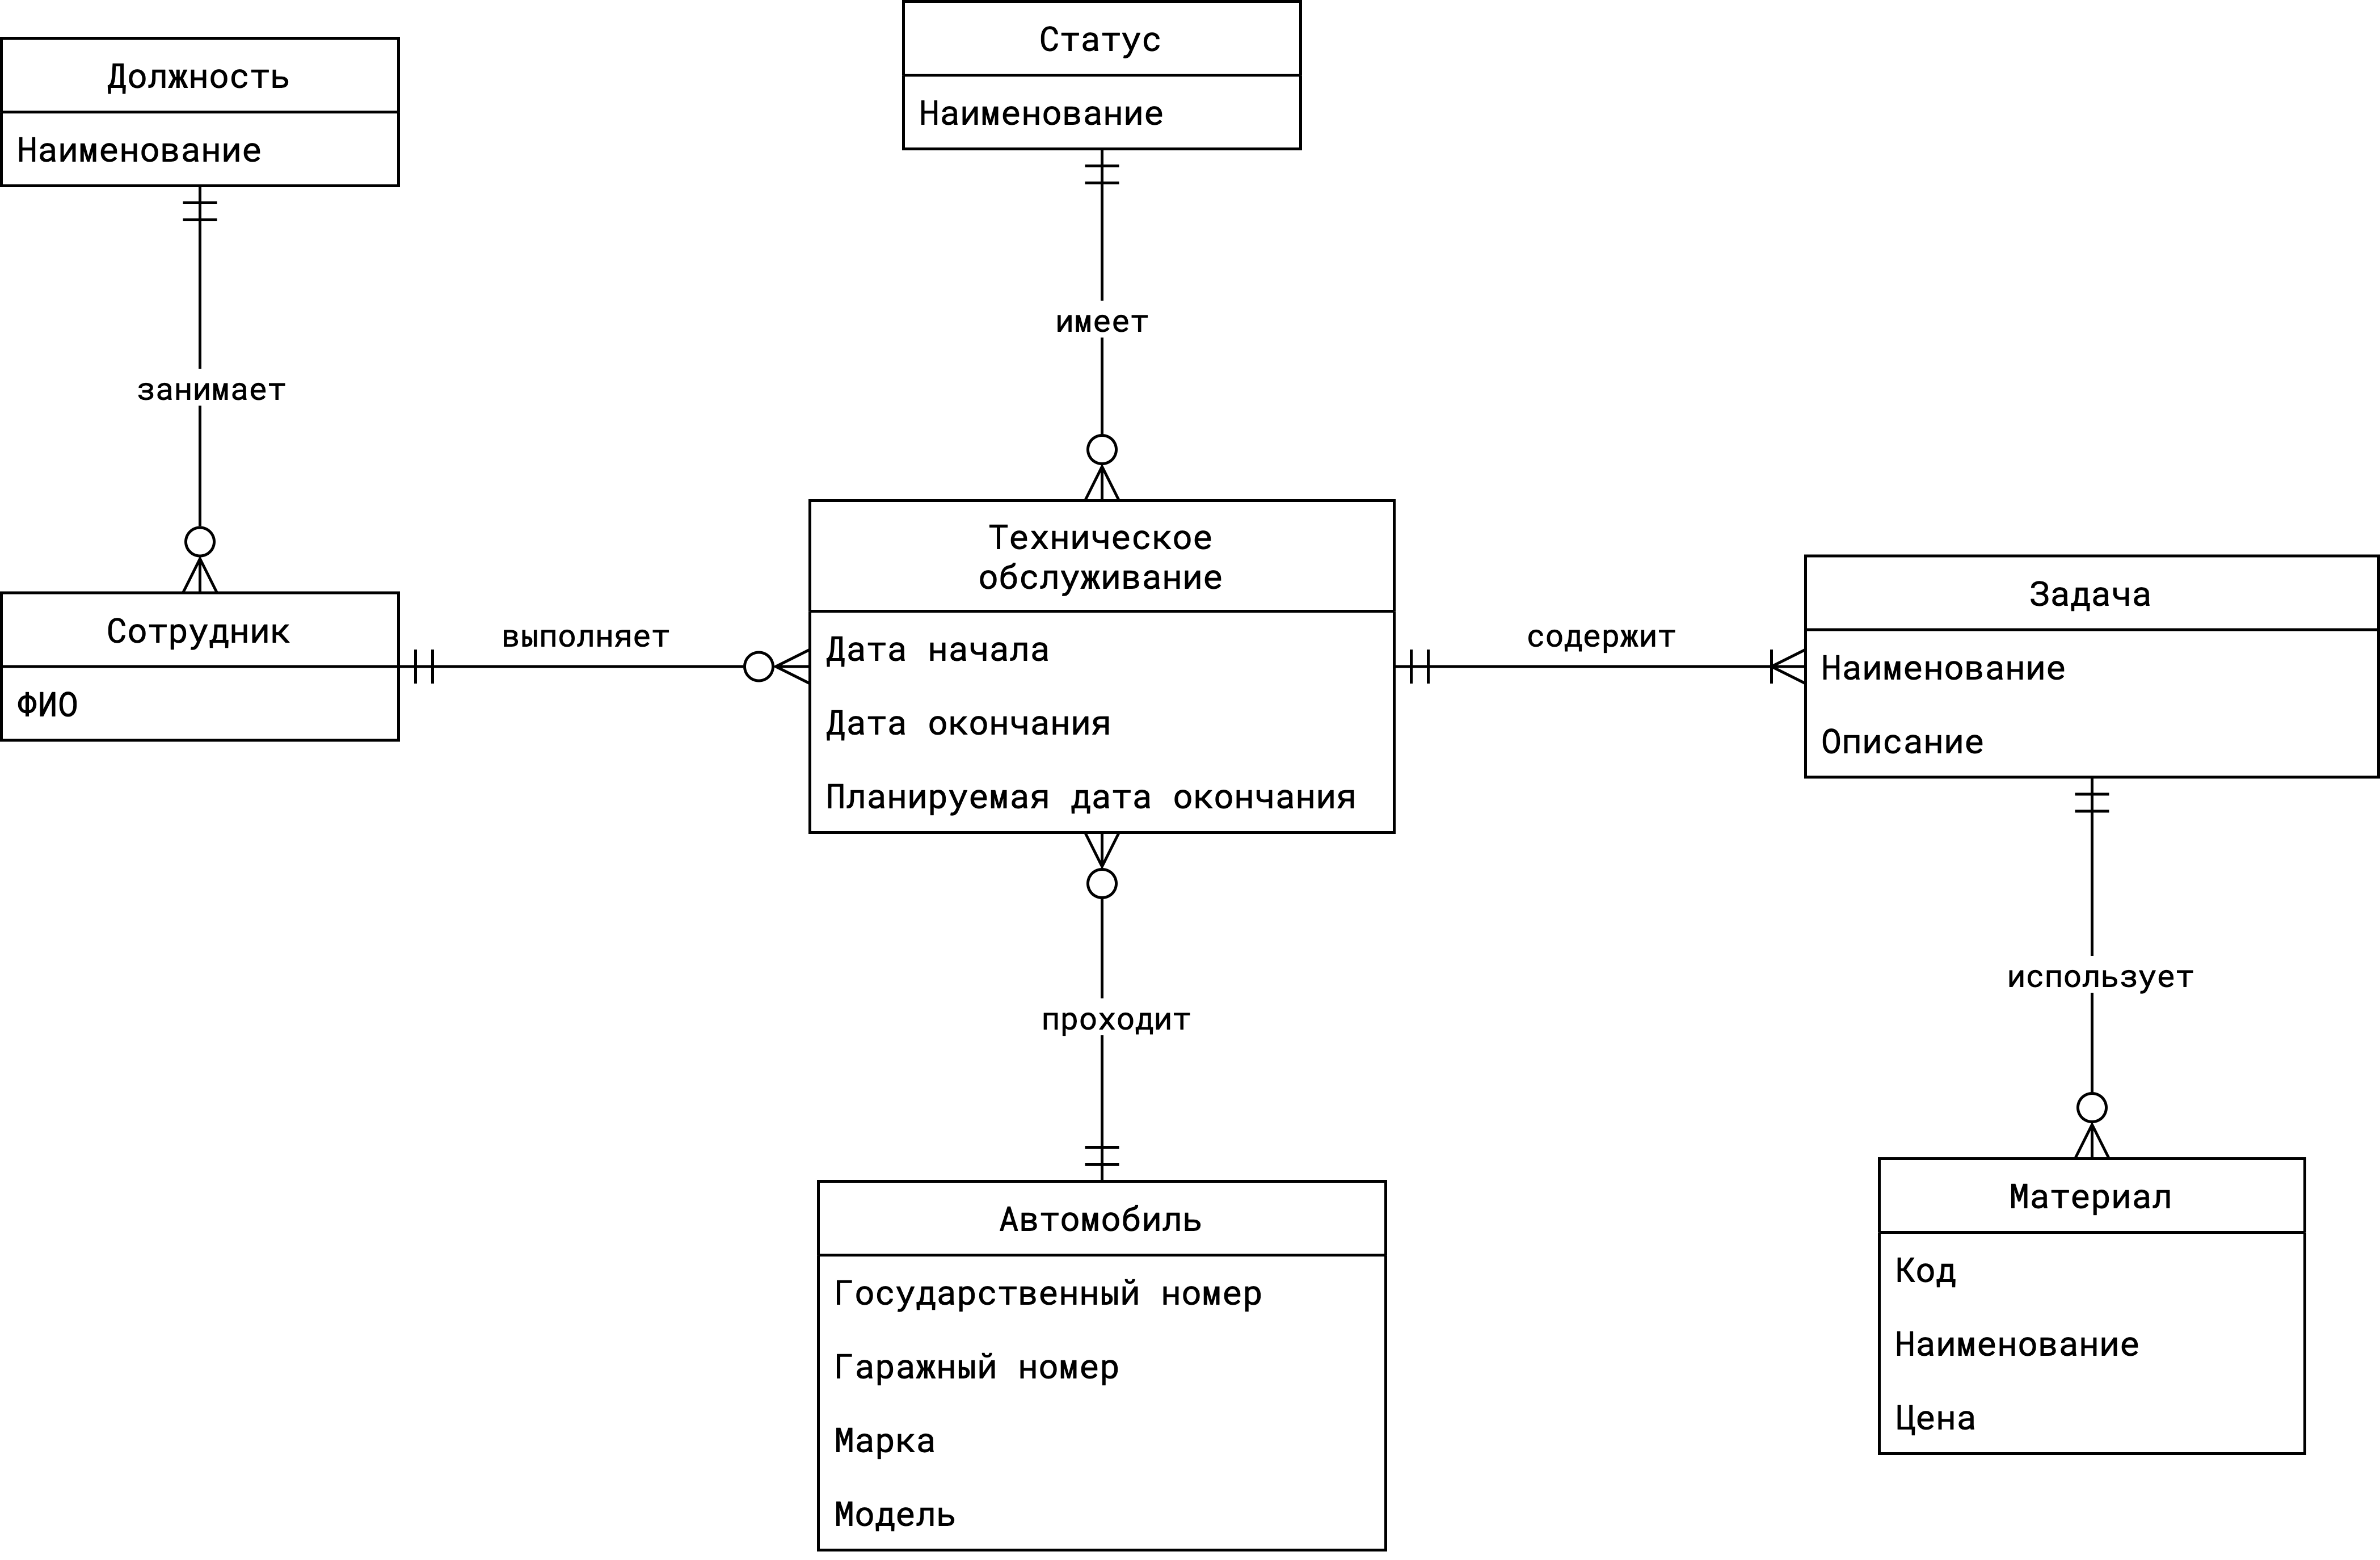
\includegraphics[keepaspectratio,width=\textwidth]{2/images/er-2.png}
        \label{fig:er-diagram}
    \end{figure}
\end{frame}

\begin{frame}
	{Теоретические математические модели}
    Стратегия для профилактируемых отказов и неисправностей
    \begin{equation*}
        d_{\text{п}} = d_{\text{к}} + k d_{\text{и}}\,,
    \end{equation*}
    {\footnotesize
        где $d_{\text{п}}$ -- стоимость ТО (профилактики); $d_{\text{к}}$ --
        стоимость контрольно-диагностической части операции ТО; $k$ --
        коэффициент повторяемости исполнительской части операции ТО;
        $d_{\text{и}}$ -- стоимость исполнительской части операции ТО.
    }
    \\[\baselineskip]
    Стратегия для непрофилактируемых отказов и неисправностей
    \begin{equation*}
        C^{II} =
        c\,/\,\bar{x} =
        c : \int_{x_{min}}^{x_{max}} x f(x)\,dx,
    \end{equation*}
    {\footnotesize
        где $\bar{x},\,x_{min} \,\text{и} \,x_{max}$ -- соответственно средняя,
        минимальная и максимальная наработки на отказ; $c$ -- разовые затраты на
        устранение отказа; $f(x)$ -- плотность вероятности наработки на отказ.
    }
\end{frame}

\begin{frame}
	{Логическая модель данных}
    \begin{figure}[H]
        \centering
        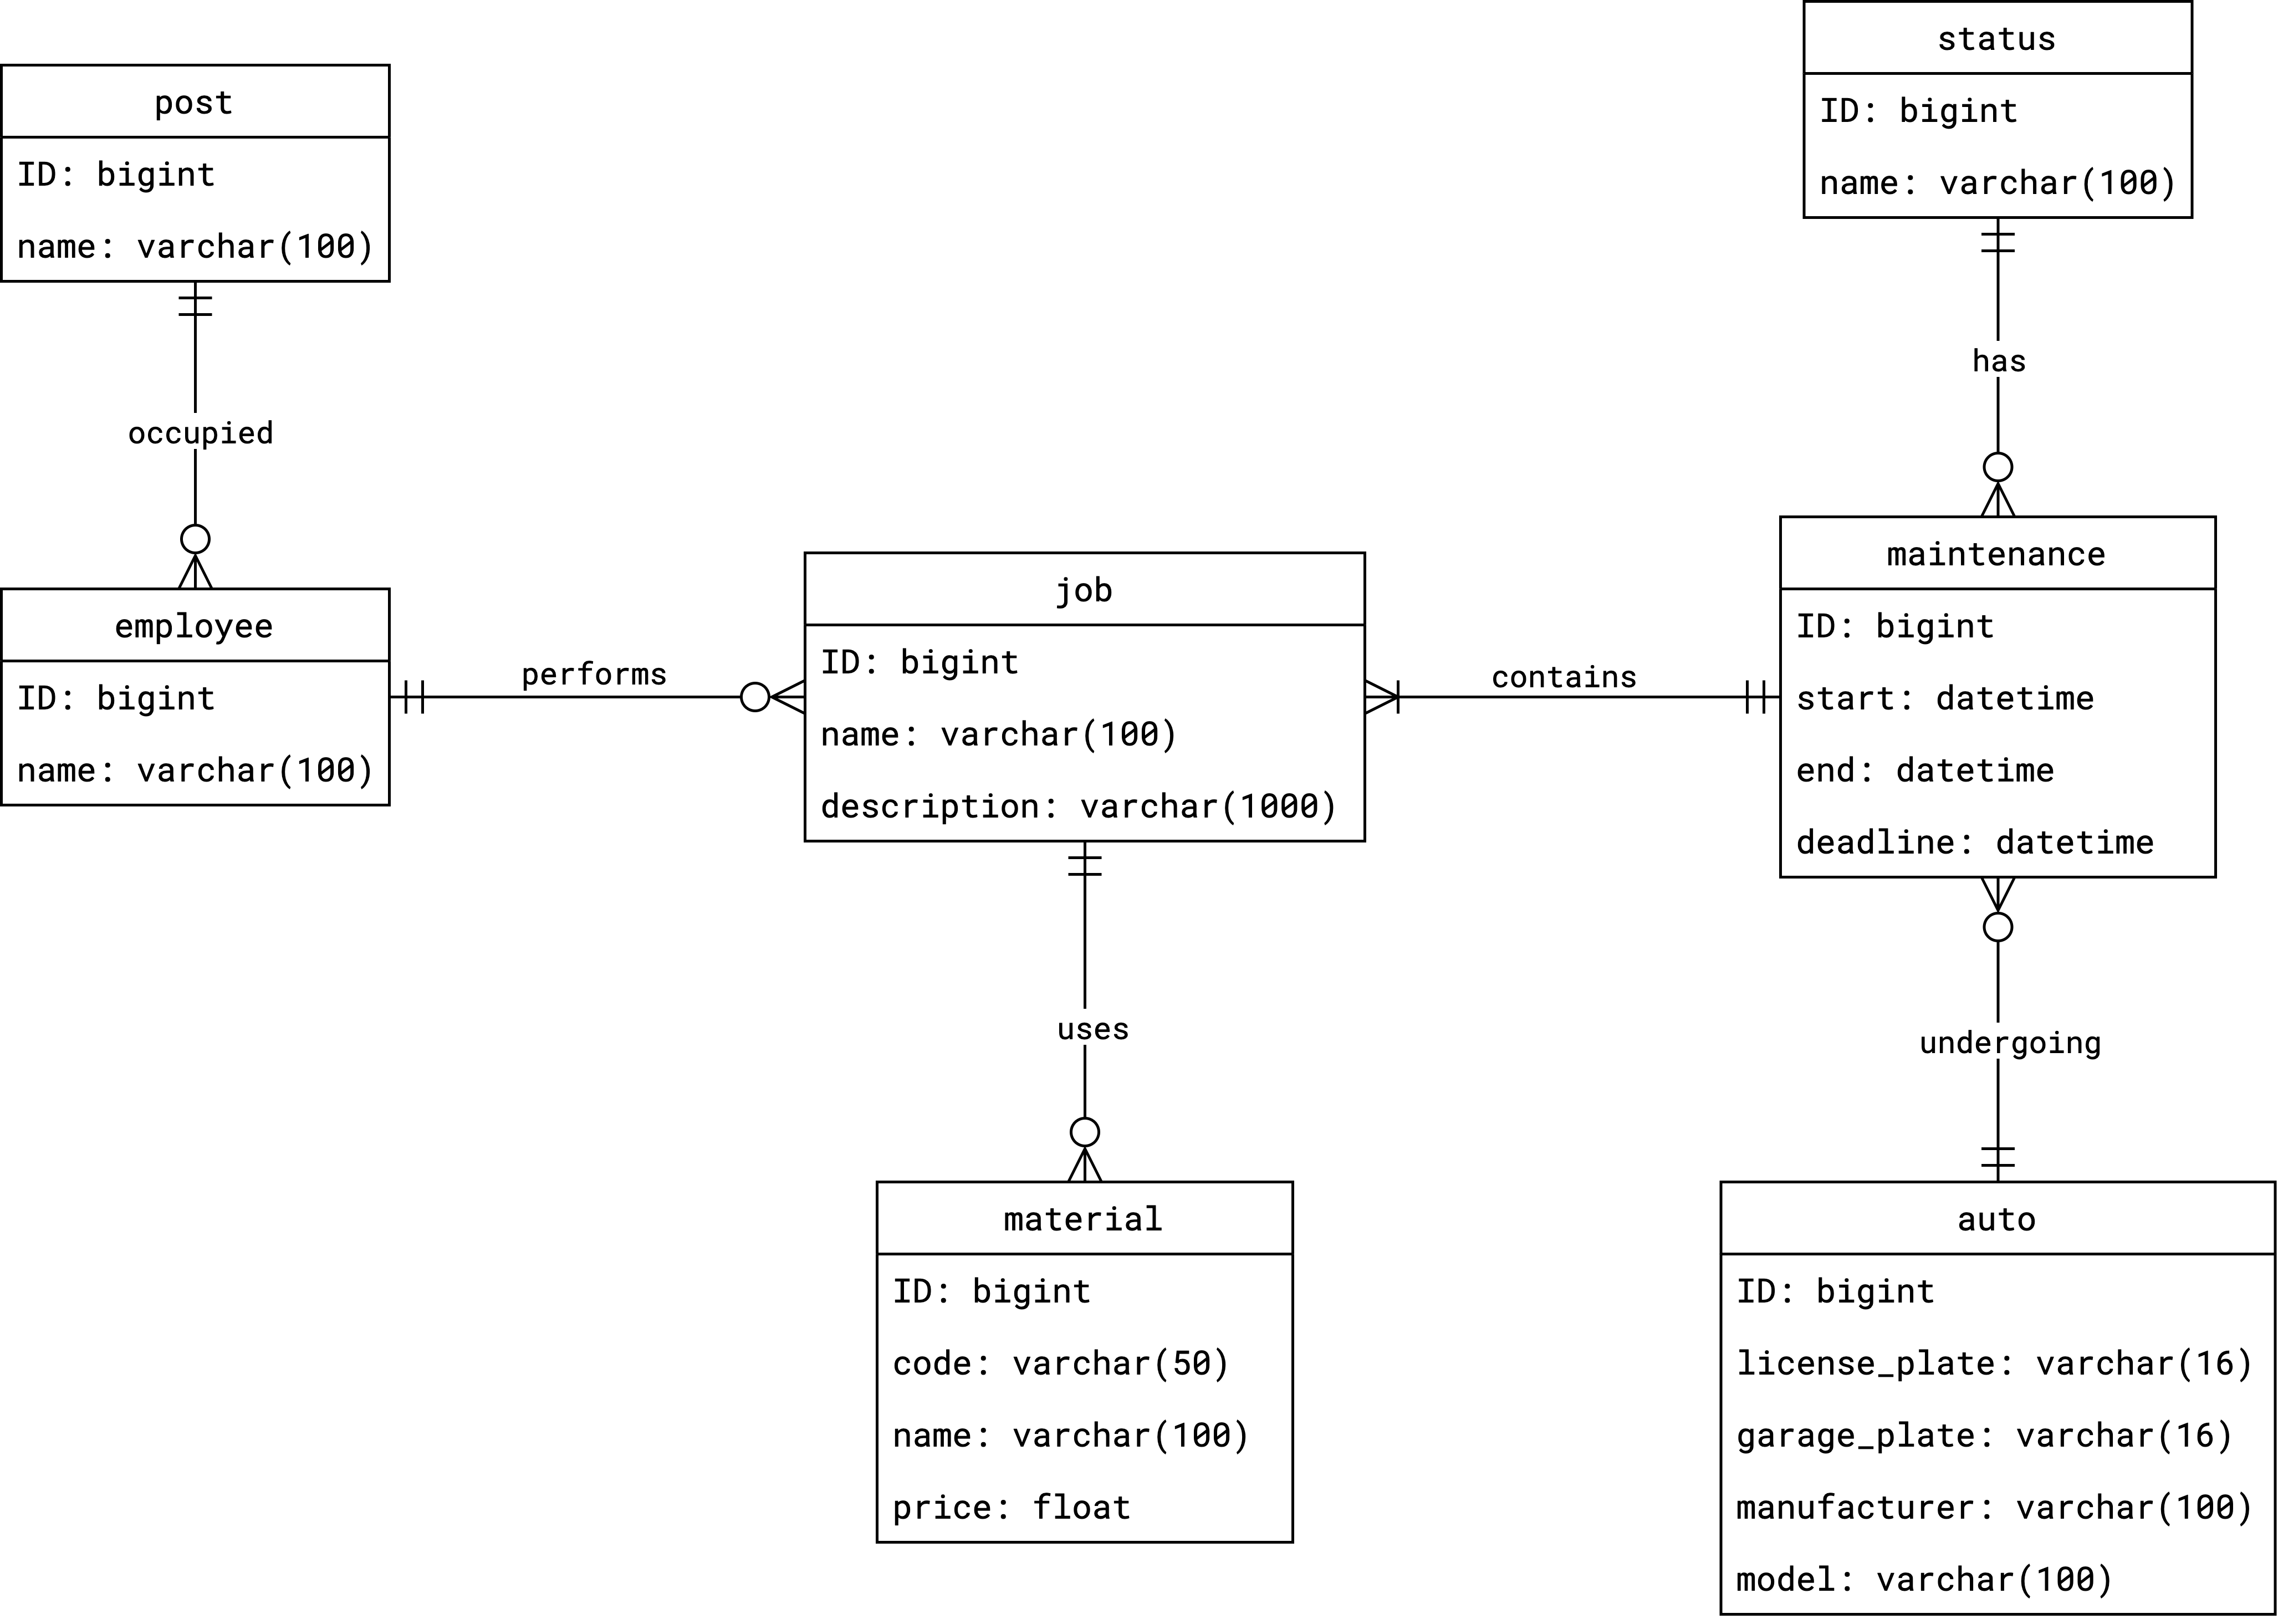
\includegraphics[keepaspectratio,width=\textwidth]{3/images/3_1_db_logical.png}
    \end{figure}
\end{frame}

\begin{frame}
	{Физическая модель данных}
    \begin{figure}[H]
        \centering
        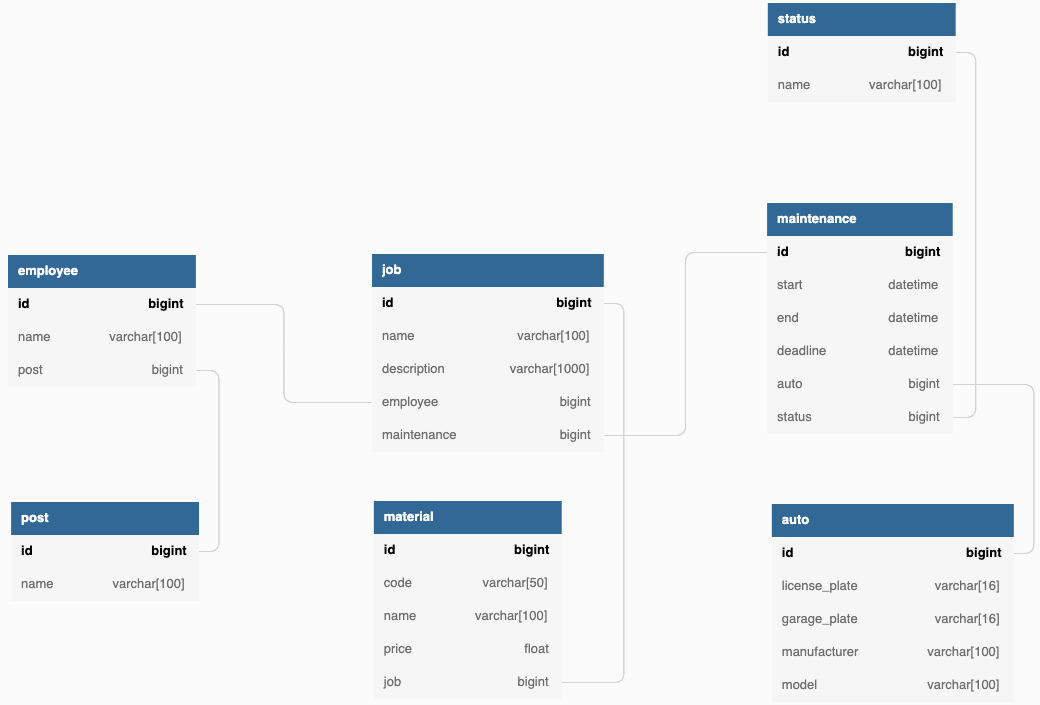
\includegraphics[keepaspectratio,width=\textwidth]{3/images/3_1_db_physical.png}
    \end{figure}
\end{frame}

\begin{frame}
	{Описание источников информации}
    Основными источниками информации в системе являются:
    \begin{enumerate}
        \item Входные данные пользователей системы, полученные от администратора,
            при их регистрации в системе.
        \item Входные данные техники, полученные из паспорта автомобиля.
        \item Информация из справочников нормативно-технической документации
            необходимых материалах для проведения технического обслуживания.
    \end{enumerate}
\end{frame}

\begin{frame}
    {Схема функционирования системы}
    \begin{figure}[H]
        \centering
        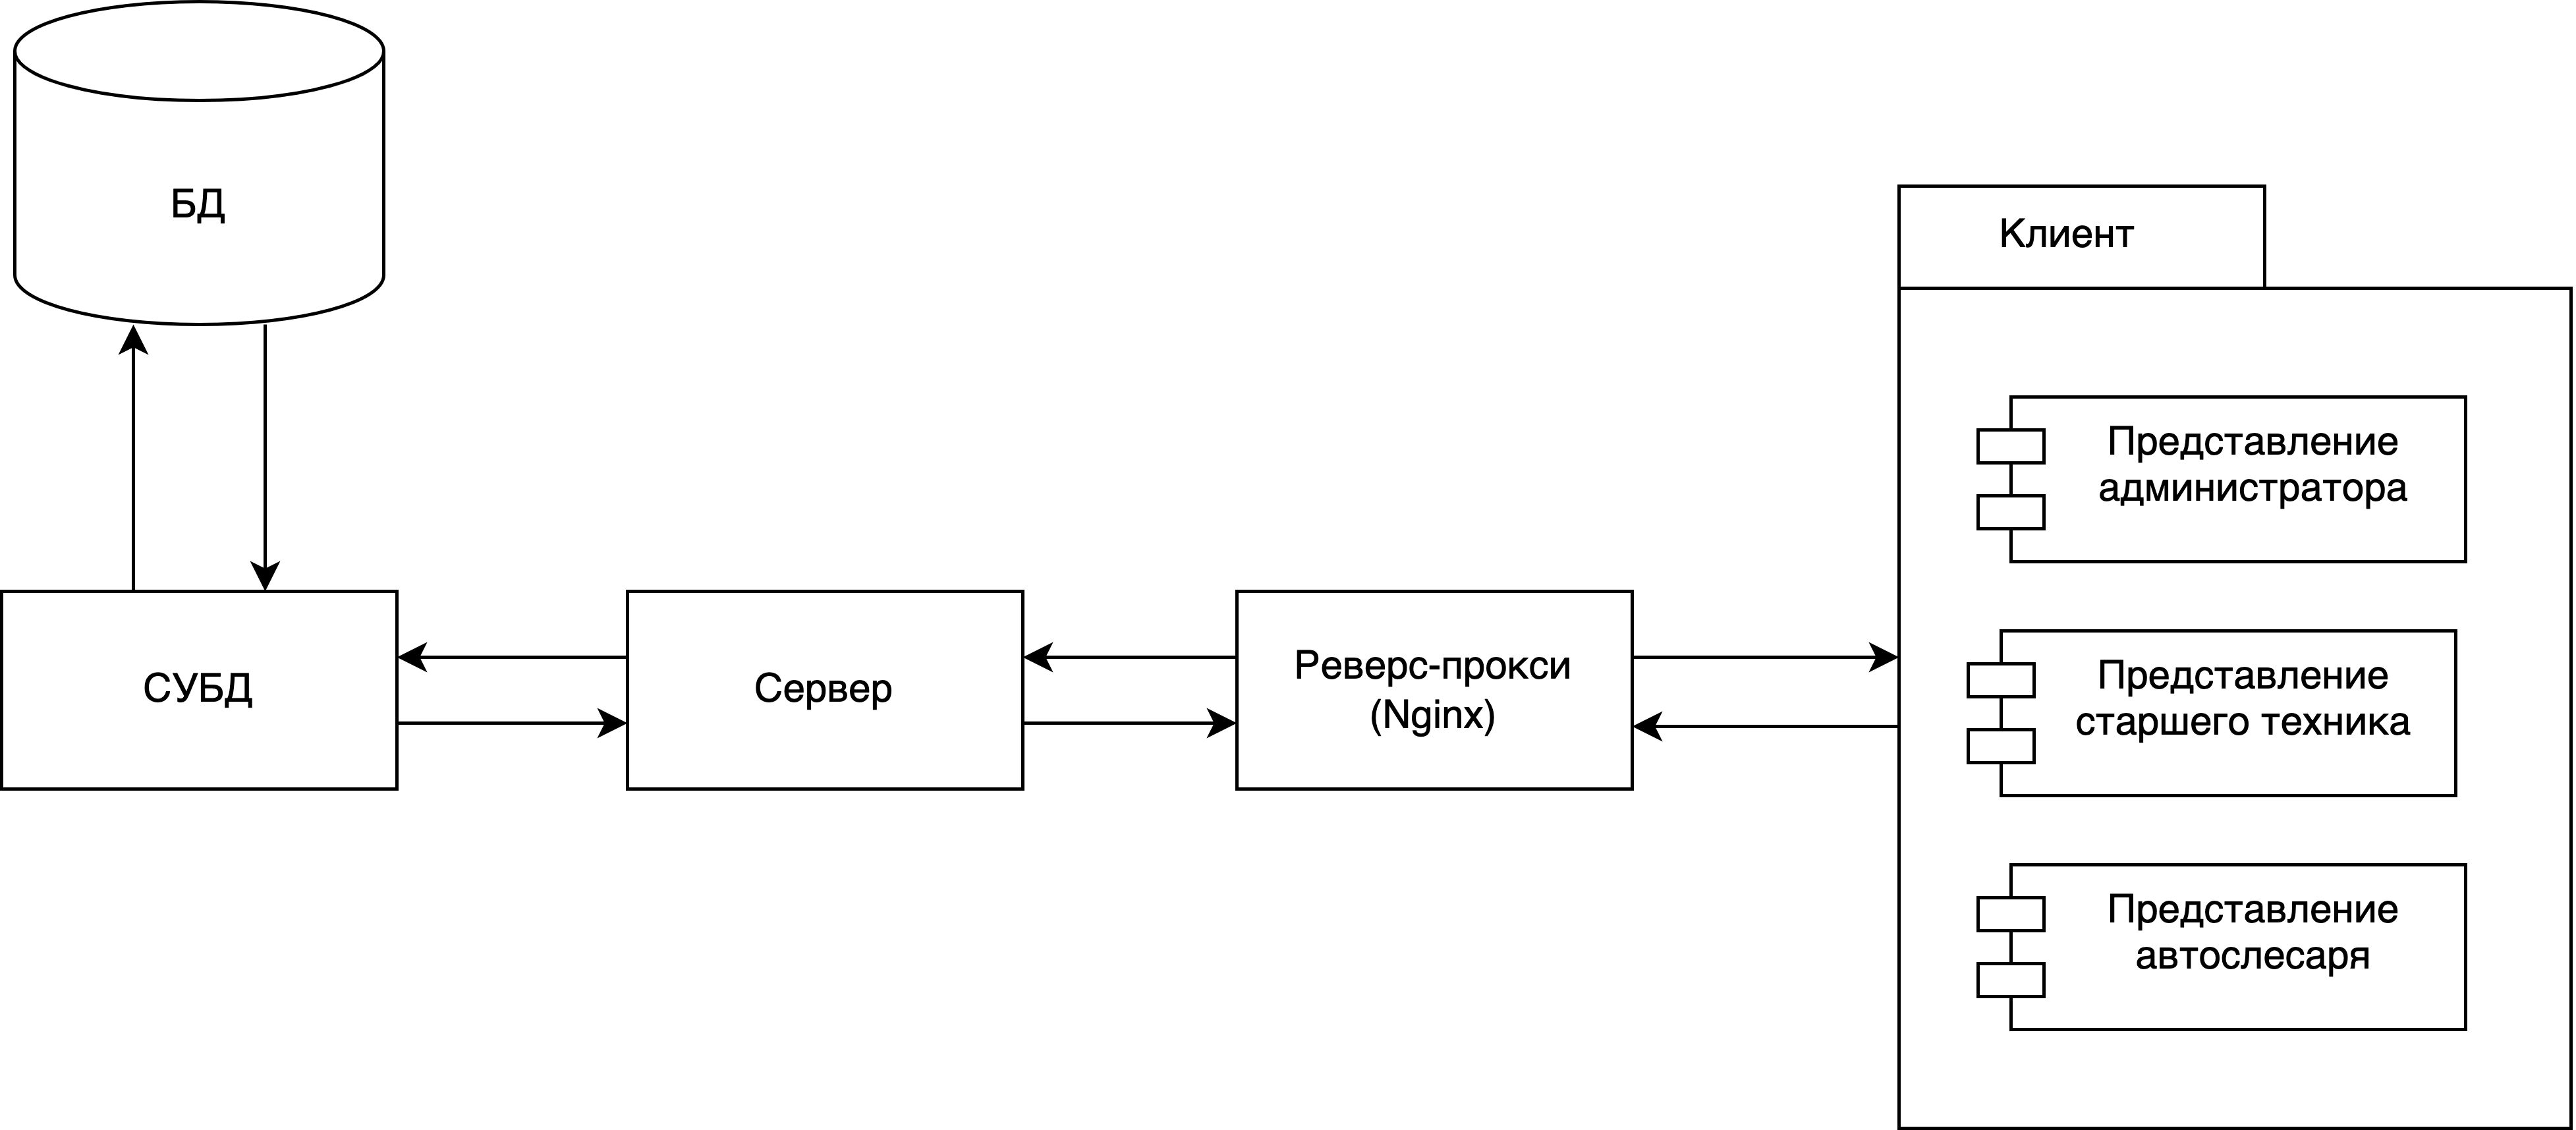
\includegraphics[keepaspectratio,width=\textwidth]{presentation/images/modules.png}
    \end{figure}
\end{frame}

\begin{frame}
    {Структура аппаратных средств}
    Минимальные системные требования для серверного приложения:
    \begin{itemize}
        \item операционная система: Windows 11, Windows 10, Debian Linux 10;
        \item процессор: с тактовой частотой 1 Гц или выше, с поддержкой
            виртуализации;
        \item оперативная память: 1Гб;
        \item стабильное интернет подключение;
        \item минимальное место на диске 2Гб.
    \end{itemize}
    \\[\baselineskip]

    Минимальные системные требования клиента -- современный веб-браузер.
\end{frame}

\begin{frame}
    {Структура программных средств}
    Для корректной работы системы требуются следующие программные средства:

    \begin{itemize}
        \item установленная система Windows 10 x64 (64-bit),
            Debian Linux x64 (64-bit) версии 10 или новее;
        \item Docker Engine v20.10;
        \item СУБД PostgreSQL 9 или новее;
        \item веб-сервер Nginx v1.10 или новее.
    \end{itemize}
\end{frame}

\begin{frame}
	{График прохождения технического осмотра}
    \begin{figure}[H]
        \centering
        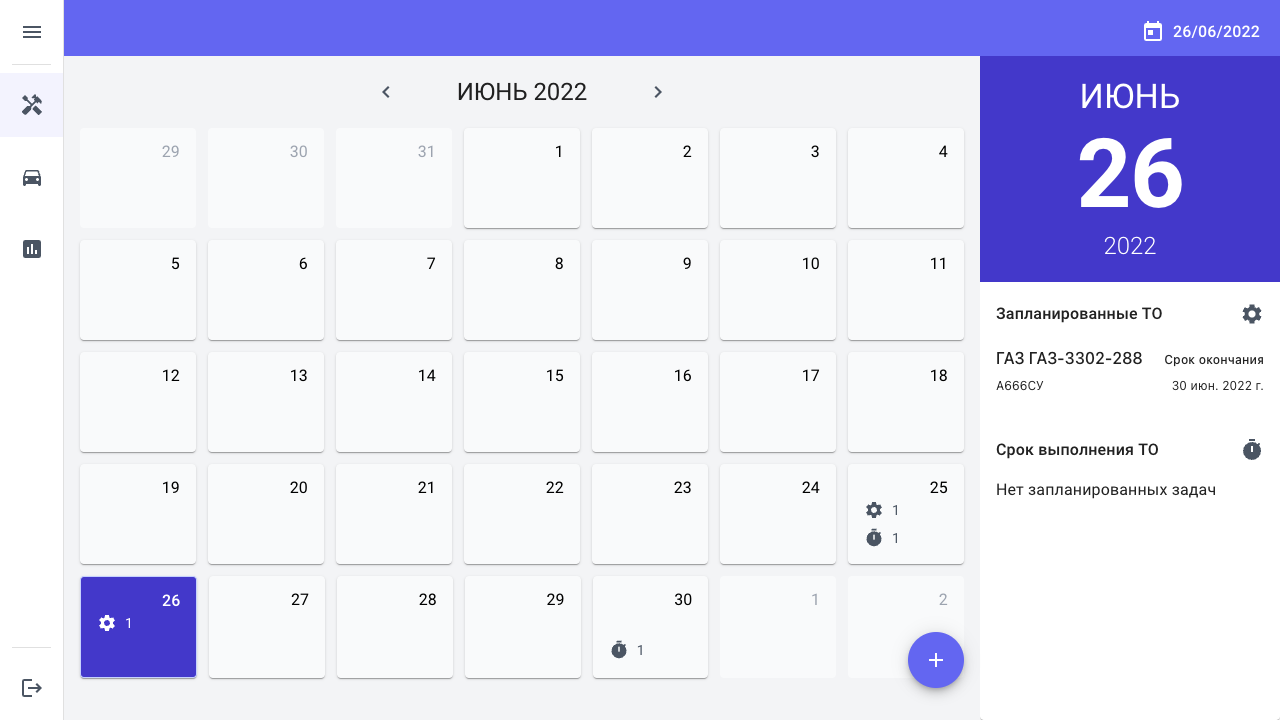
\includegraphics[keepaspectratio,width=\textwidth]{presentation/images/tech.plumpalbert.xyz.calendar.png}
    \end{figure}
\end{frame}
\begin{frame}
	{Добавление технического обслуживания}
    \begin{figure}[H]
        \centering
        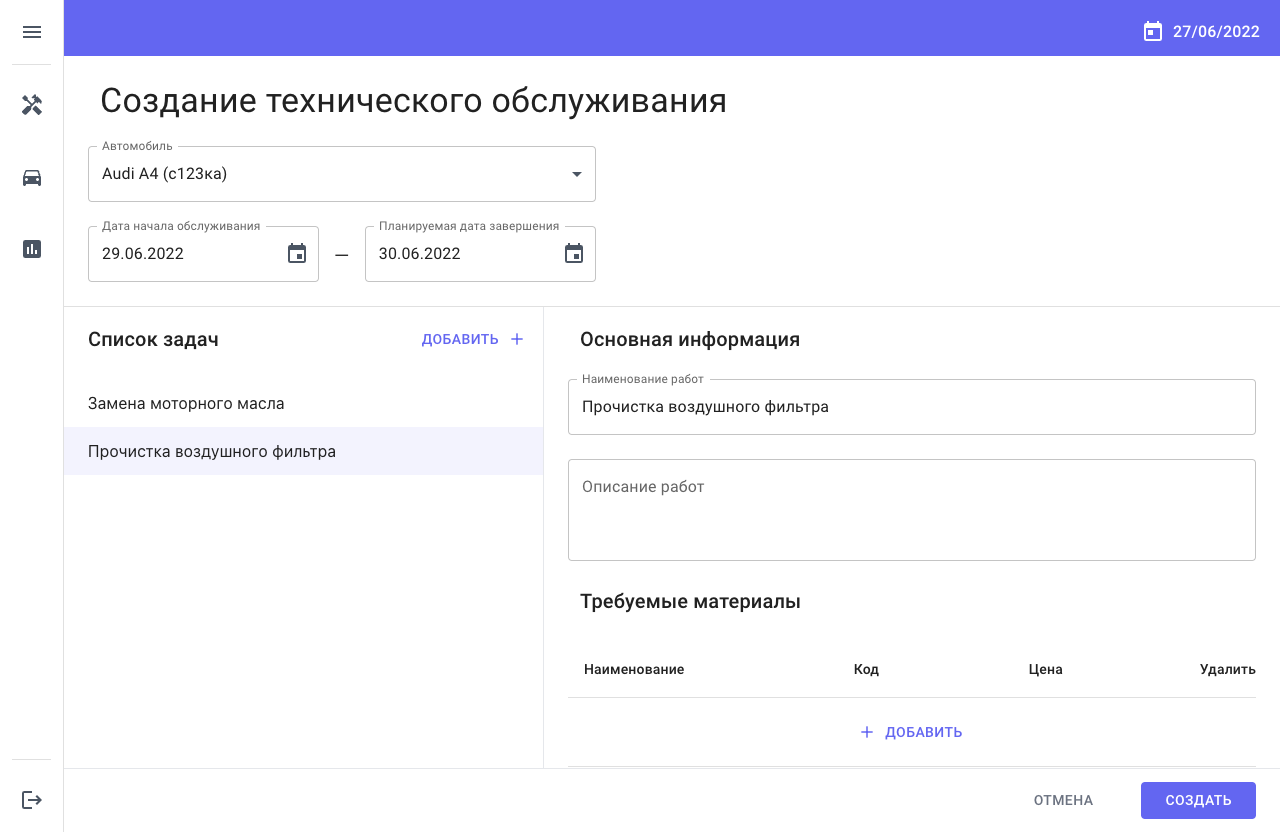
\includegraphics[keepaspectratio,width=\textwidth]{presentation/images/tech.plumpalbert.xyz.create_maintenance.png}
    \end{figure}
\end{frame}
\begin{frame}
	{Отчеты по затратам}
    \begin{figure}[H]
        \centering
        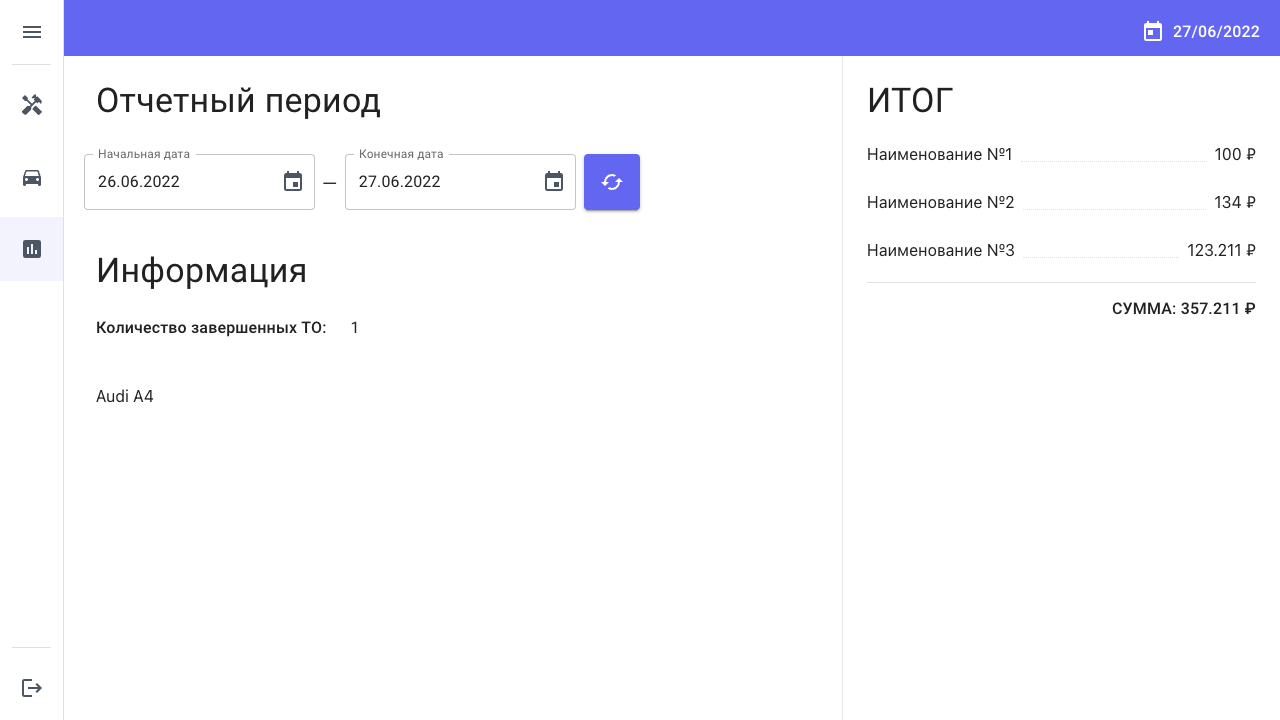
\includegraphics[keepaspectratio,width=\textwidth]{presentation/images/tech.plumpalbert.xyz.report.png}
    \end{figure}
\end{frame}
\begin{frame}
	{Парк автомобилей, зарегистрированных в системе}
    \begin{figure}[H]
        \centering
        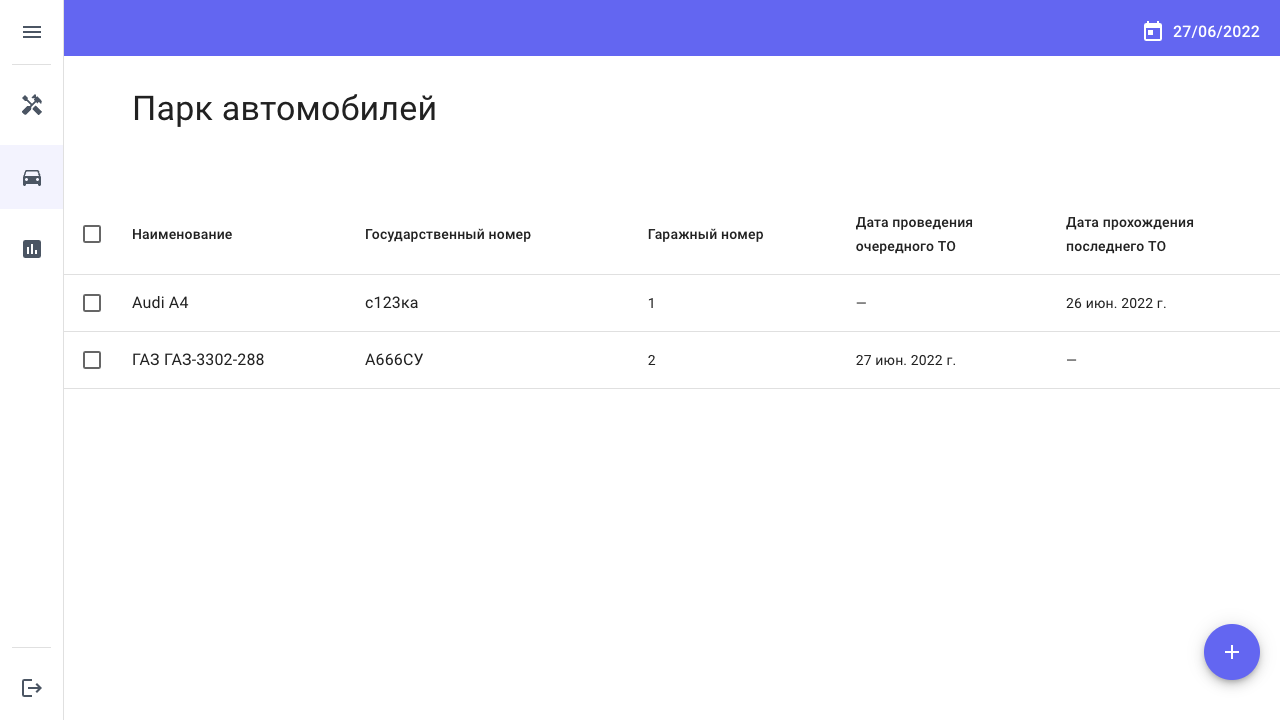
\includegraphics[keepaspectratio,width=\textwidth]{presentation/images/tech.plumpalbert.xyz.autos.png}
    \end{figure}
\end{frame}
\begin{frame}
	{Список активных обслуживаний автослесаря}
    \begin{figure}[H]
        \centering
        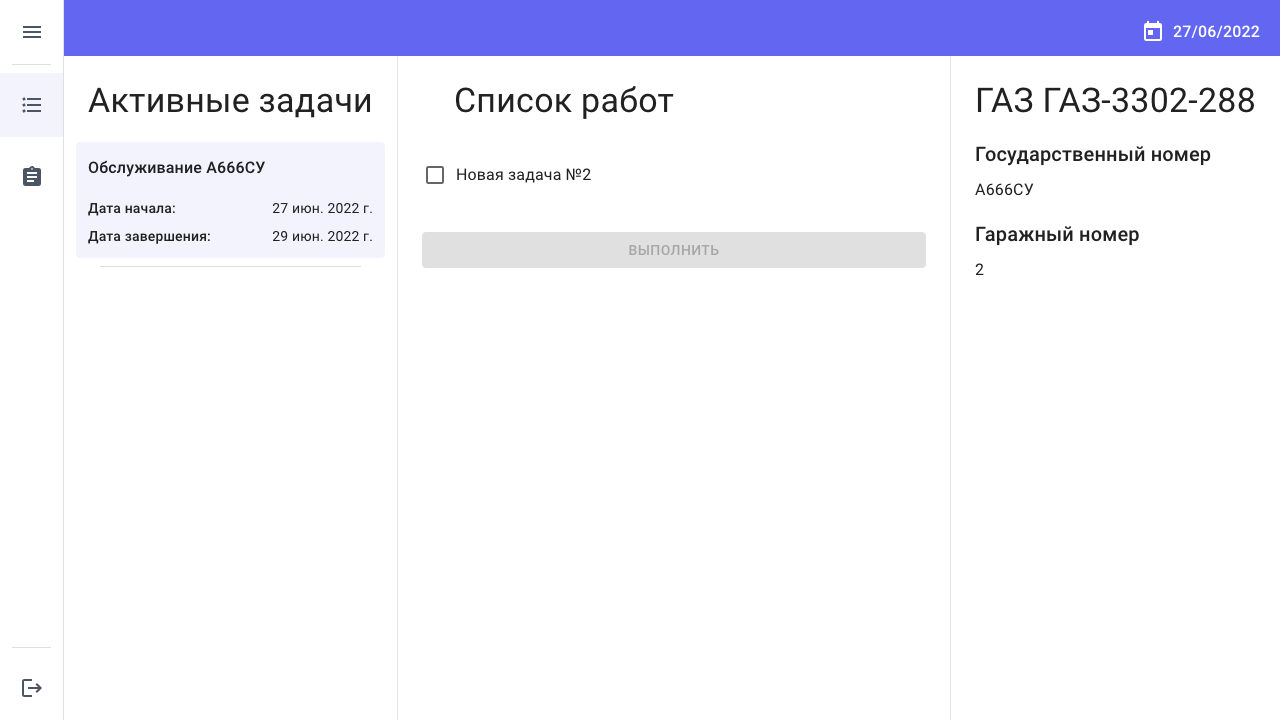
\includegraphics[keepaspectratio,width=\textwidth]{presentation/images/tech.plumpalbert.xyz.tasks.png}
    \end{figure}
\end{frame}
\begin{frame}
	{Список запланированных обслуживаний}
    \begin{figure}[H]
        \centering
        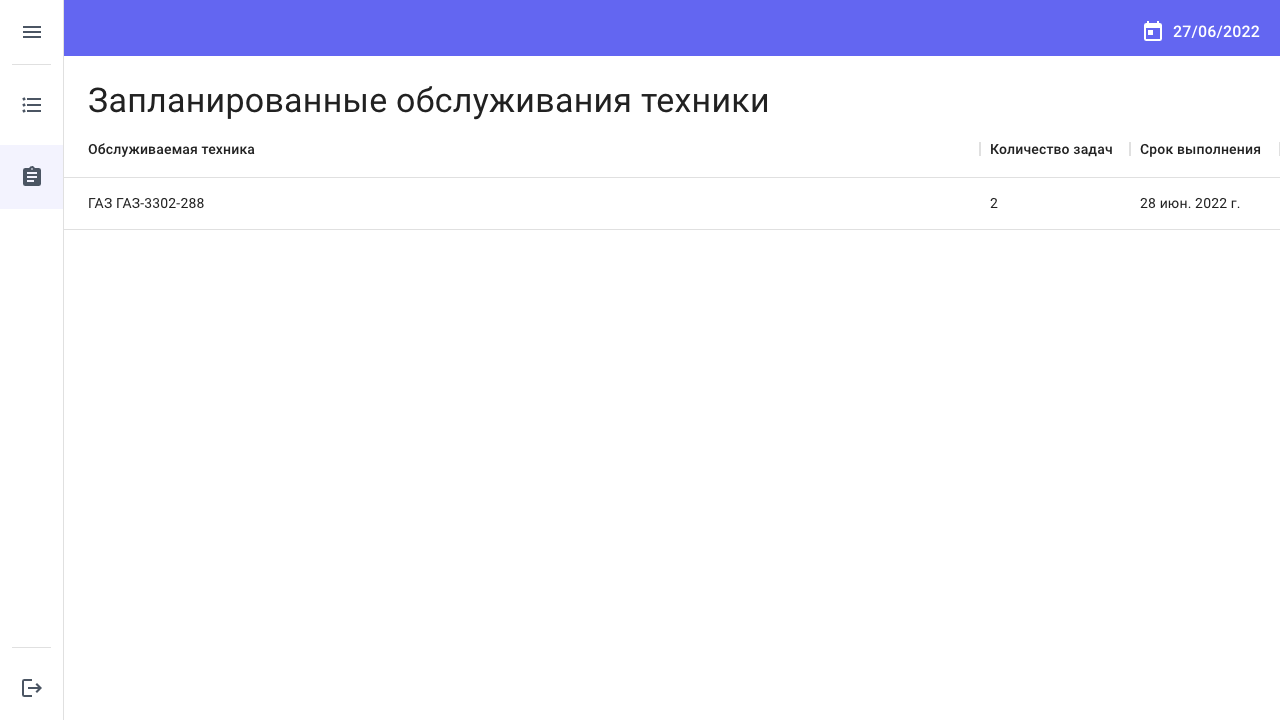
\includegraphics[keepaspectratio,width=\textwidth]{presentation/images/tech.plumpalbert.xyz.maintenances.png}
    \end{figure}
\end{frame}

\begin{frame}
    \centering
    \huge{Спасибо за внимание!}
\end{frame}

\end{document}
